\documentclass[a4paper, 11pt]{article}
\usepackage{graphicx}
\usepackage{amsmath}
\usepackage[pdftex]{hyperref}

% Lengths and indenting
\setlength{\textwidth}{16.5cm}
\setlength{\marginparwidth}{1.5cm}
\setlength{\parindent}{0cm}
\setlength{\parskip}{0.15cm}
\setlength{\textheight}{22cm}
\setlength{\oddsidemargin}{0cm}
\setlength{\evensidemargin}{\oddsidemargin}
\setlength{\topmargin}{0cm}
\setlength{\headheight}{0cm}
\setlength{\headsep}{0cm}

\renewcommand{\familydefault}{\sfdefault}

\title{Machine Learning 2015: Project 1 - Regression Report}
\author{mwurm@student.ethz.ch\\ rimartin@student.ethz.ch\\ ADDME@student.ethz.ch\\}
\date{\today}

\begin{document}
\maketitle

\section*{Experimental Protocol}
This is the protocol of the group "I don't care".

\section{Tools}
For our approach we used Python in combination with numpy and the machine learning library "scikit-learn" ~\cite{scikit}. Like this, Python offers an API comparable to Matlab ~\cite{matlab}, and it offers functionality, which is very useful for the project.

\section{Algorithm}
After trying out several algorithms we finally stick with the Random Forest Estimator of scikit-learn. Although the class of decision tree algorithms, this algorithm belongs to, has not been mentioned in the lecture yet, this class contains rather easy to understand algorithms which tend to return good results.
We used Random Forest Regressor which is a perturb-and-combine technique. It operates by constructing multiples decision trees in the training process and outputs the mean regression of the individual trees.
The deeper the tree becomes, the more complex the decision process will be, and the better the data will be fitted. By using this approach, heavy preprocessing of the data is not mandatory.

\section{Features}
Features are preprocessed performing MinMax Normalization.

Concerning features transformation we added additional dimensions to perform polynomial regression. Unfortunately, adding additional degrees to all dimensions did not lead to an improved result. We also tried to study the correlation between pairs or triplets of features and the output but we were not able to improve our model.

Feature selection was another important part. Given fourteen dimensions, it is reasonable to assume that some of them are not relevant or redundant. Furthermore variable selection enhances the generalization properties of the model by reducing over fitting. The function SelectKBest estimates the influence of the single dimensions. Then it drops all, but the k leading ones. Like this we got the best results.


\section{Parameters}
The parameter estimation is of course an important part for the random forest algorithm. Based on decision trees, the results can be unstable because small changes can end up in a completely different decision tree. To get a better overview, we first tried the method with a small set of parameters. We quickly recognized that the sequential recompilation and execution of the test, would take an enormous amount of time. Therefore the program has been optimized to enable a higher performance.
Scikit-learn has already all necessary features included. The included GridSearchCV function runs a cross validation based, fitting-performance test over all combinations of possible parameters, which are given in a separate list. The cross validation makes it possible to immediately estimate the precision of a certain configuration. The whole process from Feature Selection, over transformation to the fitting of the regressors can be combined within a single "Pipeline". Like this, the GridSearch can not only be applied to the selection of regressor parameters, but also to the selection of the amount of interesting features.
To make it possible to search a huge grid, performance is an important issue. Due to the fact, that all grid executions are independent, parallelization is fortunately easily possible (and also supported by the scikit implementation). To take the most out of this fact, the easily accessible BRUTUS cluster of ETH ~\ref{fig:brutus}, was a welcome possibility to execute the script.
\begin{figure}	
	\centering
	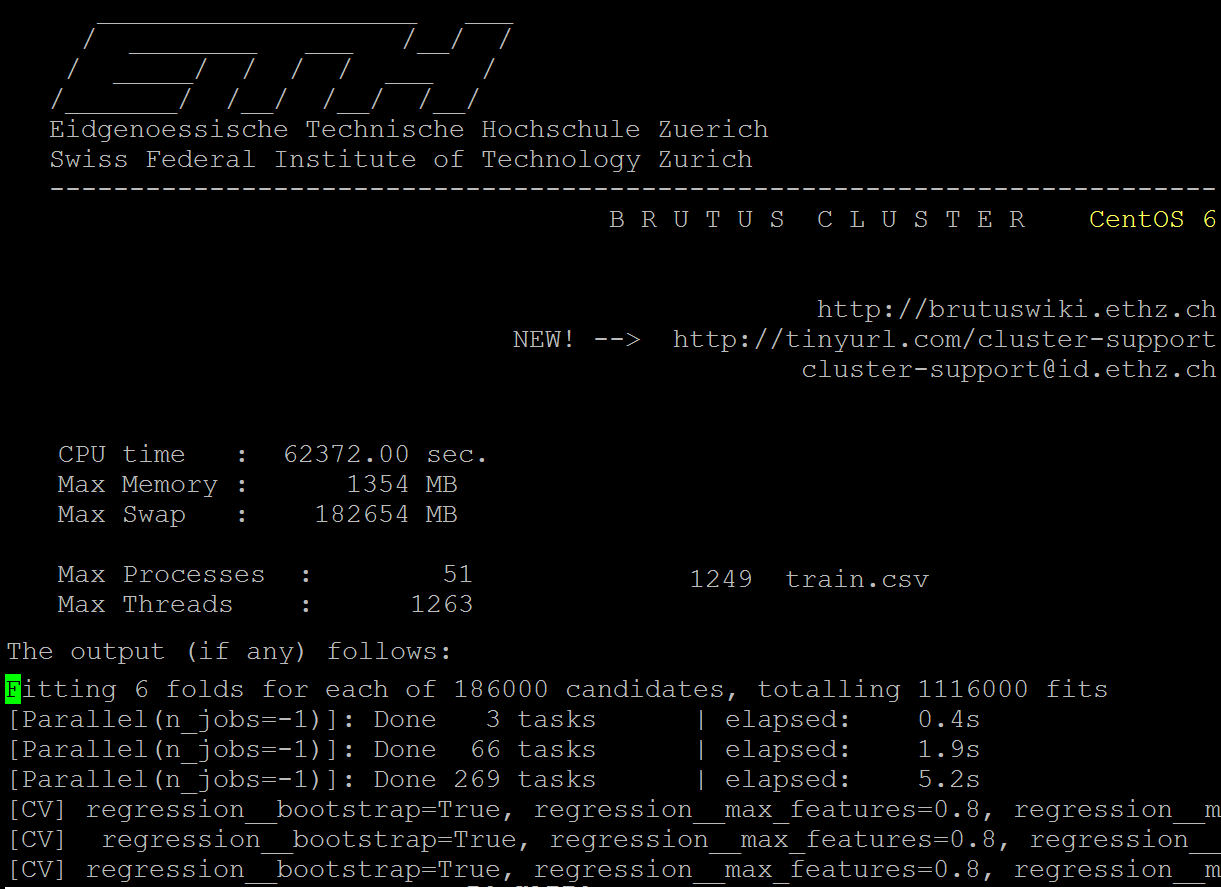
\includegraphics[scale=0.6]{ScreenshotCluster.png}
	\caption{BRUTUS cluster}
	\label{fig:brutus}
\end{figure}
The best result has been then choosen as submission.

\section{Lessons Learned}
In the beginning of the project we implement the different linear regressors mentioned in the lectures without using libraries. Then we switch to library functions and the RandomForestSelector gave the best results. Nevertheless we think, that in the end, linear methods could outperform the decision tree approach if the inherent structure of the data would be much more involved into the fitting process. Adding features is an important case in this situation. The given data comprises multiple dimensions, which can be seen as classes, because the values are limited to a small set of values, for example 2,4,8. The transformation of these classes into real classes would definitely result in a much better result. Unfortunately, there is not enough time to implement this.

\begin{thebibliography}{1}
	
	\bibitem{scikit}
	\newblock Scikit-learn Homepage 
	\newblock
	\url{http://scikit-learn.org}
	
	\bibitem{matlab}
	\newblock Matlab Homepage
	\newblock
	\url{http://www.mathworks.com}
	
\end{thebibliography}

\end{document}

